\chapter{Understanding}

\begin{quote}
It isn't that they can't see the solution. It's that they can't see the problem.
\attrib{Gilbert K. Chesterton}
\end{quote}

- cognition is relative; metaphor



\section{Perspective Collection}

\begin{quote}
A good stack of examples, as large as possible, is indispensable for a thorough
understanding of any concept, and when I want to learn something new, I make it
my first job to build one.
\attrib{Paul Halmos}
\end{quote}

I know a bit of abstract algebra. And I know how to cook. It turns out, cooking
has gotten me a lot more attention from women than cooking ever has -- who knew,
right? (Don't answer that.)

You know, the two subjects have a lot in common. And I don't mean this in some
deep, ``the reality of the universe is contained in mathematics and mathematics
is contained in the reality of the universe'' babble. Maybe symmetry in recipes
makes them taste better. I don't know.

You'll need a more informed mathematician to speak about that.

What I mean is that learning either of these subjects can teach you the same
lesson about human cognition. That lesson? \textbf{Collect multiple
  perspectives.}

When I want to cook something, I never read just one recipe -- I read five or
ten. With five or ten recipes, you can pattern match. Ask yourself, ``What's
constant across all of these recipes?'' And once you know the answer to that,
well, you've sort of just figured out the heart and soul of a dish.

Wittgenstein can argue all he wants about the definition of a game but, read 5
recipes for the same thing, and you'll have a definition of that dish. And you
don't even need some platonic cookbook sent down from on high. All you need is
an internet connection.

Once you understand the core of a dish, you're free to improvise. And I think
that's really what cooking is about. Grasping the underlying pieces of a recipe
that make it \textit{it} and then adding your twist to it. A delicious cinnamon
twist, maybe.

Abstract algebra works in the same manner. If you want to know what a field,
group, or a monoid is, you can't just read one recipe, one treatment. You need
to read five or ten. Flip through a dozen textbooks. Once you've deciphered those, you ought to have a good
idea about the object in question.

Or take mathematical proof, for instance. What's the point of knowing multiple
proofs for the same theorem? Why, once something has been proven, do
mathematicians continue searching for cleaner, more elegant proofs? Or proofs by
different means? Maybe more elementary ones.

Why bother? It's been proven. It's valid. Who cares?

The purpose of multiple proof, and even mathematical proof in general, is not to
erect the truth of something in such a way that it's impervious to sane
criticism. That's just a side effect.

The real point of a proof is to illuminate the mathematics -- we're after
insight, not correctness guarantees. And that's the point of multiple proofs:
each, if we're lucky, sheds some additional light on the structure. Our mental
picture becomes sharper, more defined.

We start to feel that we know.

So we've generalized this from recipes, to abstract algebra, to math and proofs
as a whole, but don't stop there: \textbf{to understand anything, anything at all, in
  any significant way, collect perspectives on that thing}.

5, 7, 13. The number of perspectives you need varies. With something simple,
maybe none are needed. With something complex, maybe you need to read 100 takes
on the same idea.

In fact, this idea is so powerful that it's not limited to humans. Hell, it's
not even limited to organic life. There have recently been some advances in
automated theorem proving by training programs on several different proofs of
the same theorem -- exactly the idea I've just told you about.

% tk find link/citation

\section{Debugging Confusion}
\begin{quote}
A person taking a test or playing a piece of music is executing a program, a
deterministic procedure.  If your program has a bug, then you'll get a whole
class of problems wrong, consistently.
\attrib{celandine13, \href{http://celandine13.livejournal.com/33599.html}{the most insightful LiveJournal entry of all time}}
\end{quote}

Lend me your imagination for a minute.

One day, you're cleaning your attic. Light filters in through some crooked
blinds. It highlights the (significant) dust in the air, and you can make out
each speck, like a tiny alien race, come to colonize your attic. 

It's hot. You wonder why you volunteered for this project in the first place.

You're emptying a chest of drawers and you stumble across... well, it's what
looks like a glass sphere -- sorta a snow globe, but sans base.

It has to be old, given the amount of grime that it's accumulated. The muck
coats your fingers. Your nose curls and you grimace in a moment of disgust, and then you grab a
towel -- first each finger, and then you polish off the mutant snow
globe.

And, as it starts to gleam, your attention latches onto the tiny glass planet,
until, with a start, you realize that you can't feel your body. It's like your
consciousness has been possessed, and you can't steal your eyes away from the
ball.

Bit by bit, the attic around you disappears like television static, and you find your awareness floating,
bodyless, over a boy hunched over a math problem set and a sheet of paper. He
grips a pencil and, by his side, there lies the nub of what used to be a meaty
eraser.

As he flips through the back of the calculus book, the look of concentration on
his face is replaced with one of expectation. He lands on a page. 

His fist strikes the table.

There's a frustrated bellow-grunt, and you hear him say, "I'm too stupid. I'll
never get this."

You, too, are swept away in a moment of shared frustration, as your mind is
doubly hijacked: first by the snow globe, and now by empathy.

You wonder why the ball has sent you here, to this particular time and place,
and then...

\section{What's in a skill? }

Here's something I dislike: when people describe something as algorithmic as an
insult. Oh, \textit{that}, it's so algorithmic. A computer could do that.

Like when colleges tout that oh, well, we have humans review each child's
application, unlike some other places, who just let a \textit{computer} do
it.

Except, when you look at the empirical data, it's very, very tough to find a
situation where a human's predictive ability beats out a computer. 

This is well-documented in Robyn Dawes's landmark paper, "The robust beauty of
improper linear models in decision making." The gist of the paper? Basically,
even ghetto,
if-they-were-FDA-regulated-only-Chinese-citizens-would-be-allowed-to-buy-them
models outperform human.

\begin{quote}
This article presents evidence that even such improper linear models are
superior to clinical intuition when predicting a numerical criterion from
numerical predictors. 
\end{quote}

This paper could be considered the precursor to Tetlock's magnum opus, \textit{Expert
Political Judgment}, which found that quantitative models outperform, you know,
everyone.

This is illustrated in the book's most famous graphic, reproduced below, where
statistical models wrek the human and chimpanzee competiton.

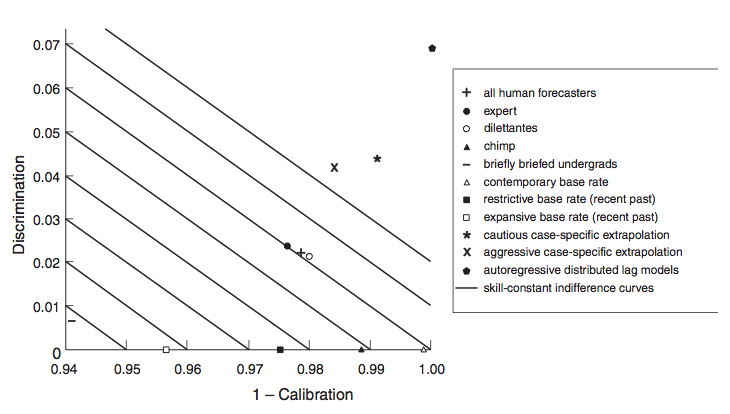
\includegraphics{expert-political-judgment}

But, right, I'm getting a little carried away here. The point I'm trying to make
is that \textit{algorithms rule}. And, like I've argued before, everything can be
described as an algorithm. The entire scientific enterprise can be described as
algorithm-hunting.

The question, "How does the mind work?" is really looking for a step-by-step
process that the mind goes through to accomplish something -- when you can write
something down in such a way that a program can do, that's when you've
understood it.

If every process can be conceptualized as an algorithm, then, skills must fall
under that umbrella -- a skill is an algorithm, or as the quote at the intro
puts it, "A person taking a test or playing a piece of music is executing a
program, a deterministic procedure."

What are errors, then? Nothing but bugs in your program.

\section{Mistakes are valuable}

Humans are handicapped by our binary notion of correctness -- the notion that an
answer on a test is either correct or not. That there are no degrees.

But, after a bit of reflection, it becomes clear that one answer can be more
correct than another, while both can still be technically wrong.

Isaac Asimov has this to say on the subject in "The Relativity of Wrong,"

\begin{quote}
[W]hen people thought the earth was flat, they were wrong. When people thought
the earth was spherical, they were wrong. But if you think that thinking the
earth is spherical is just as wrong as thinking the earth is flat, then your
view is wronger than both of them put together.
\end{quote}
  
Once we abandon the binary notion of right and wrong, the actual nature of
wrongess becomes a bit more clear -- some of the haze dissipates. You will, if
you're paying attention, notice that wrongness is not one thing.

That there are many different ways to be wrong, and each of them have
indentifiable causes and the cause, once removed, eliminates the
wrongness. Thus, the label "stupid" or "bad at" are not so much explanations, as
they are frustrated noises that, when decoded, translate to "you're getting it
wrong but I don't understand the reason why."

When I was a student, I didn't understand this about wrongness and I didn't grok
that \textit{mistakes are evidence.}

Imagine you're a teacher, and you're grading 35 tests on, say, division,
and every test comes back the same: every student has answered that 100 divided
by 10 equals 90.

Are you going to say to yourself, "Well, I guess I just got a really dumb batch
of children this year. That's why they're getting it wrong."

No, of course not. You're going to go back over division with the children, with
an emphasis on the differences between division and subtraction -- because
apparently all the kids think you're asking them to subtract!

When you're learning something on your own, you have to be that teacher. If you
get something wrong, you need to stop, and pay attention to your mistake. With
mathematics, assuming you've kept reasonable notes, you can walk through your
answer, step by step, and see at which point you went wrong.

You can zero in on the bug and destroy it.

That's the process of debugging confusion.

\begin{itemize}
\item First, you get a problem wrong.
\item Then you must infer the cause of the mistake by collecting evidence.
\item Once you have the cause of the mistake, dispel the confusion, crush the bug,
  and update your programming.
\item Repeat this process until you've dispelled all of your bugs and reach the
  correct answer.
\end{itemize}

\section{Deeper Processing}

\section{Fixed versus growth mindsets}

\begin{quote}
  If you hear a voice within you say 'you cannot paint,' then by all means
  paint, and that voice will be silenced.
\end{quote}

Imagine, for a moment, that you are teleported to an alternate universe. The
year is 1891.

A 10 year-old boy named Pablo sits down in front of a piece of paper. He grips a
pencil in his right hand. On the table in front of him, an orange.

He closes one eye, concentrates on the orange, and moves the pencil across the
paper. He produces a line.

He looks at it, sighs, and gets up from the table.

The next day, the same thing happens. This goes on for weeks. Pablo's drawing of
an orange never improves. Always just a damned line.

\section{Dweck's research}

Carol Dweck has been doing research on what she calls fixed and growth
mindsets. The basic characteristic of a fixed mindset is believing that skills
and personality are not malleable -- they're fixed. You're either born good at
something or not, and that's the extent of it.

A growth mindset is the opposite: the belief that skill is something that can be
shaped through practice.

Dweck sometimes likes to present this in terms of intelligence, but I think this
is misleading. If you ask five people for a definition of intelligence, you will
get five different answers. That just confuses the issue.

Dweck should stop abusing lay notions of intelligence and just focus on skills.

As you may be anticipating, it's better for you to believe that skills aren't
fixed. Here, for instance, are the math grades of those who adopt a growth
versus a fixed view:

\graphic{fixed-vs-growth-math-dweck}

And here's what happens when students are taught a growth mindset:

\graphic{math-intervention-dweck}

Indeed, somewhat perversely, the fact that believing in a growth mindset
improves performance is evidence that a growth mindset is truer than a fixed
one: if believing you can do it improves your skills, it's hard to see in what
sense they're fixed.

And, indeed, that's the point of the Pablo parable. What would the world be like
if skills actually were fixed? No one would be able to whistle, Pablo Picasso
never would have drawn anything more than a line. Forget learning a second
language. Hell, forget learning a first language.

The point being: \textbf{Any skill can be improved with practice.}


\section{Read with the intention of teaching}
There is compelling evidence that when students read with the intention of learning the material as well as they can, they learn less than students instructed to learn the material so that they can teach it to someone else (Bargh & Schul, 1980).

\section{Paying attention}

Multi-tasking makes you stupid.

But don't take my word for it. Here it is from science's mouth:

\begin{quote}
Results show that when peripheral tasks interrupt the execution of primary
tasks, users require from 3\% to 27\% more time to complete the tasks, commit
twice the number of errors across tasks, experience from 31\% to 106\% more
annoyance, and experience twice the increase in anxiety than when those same
peripheral tasks are presented at the boundary between primary tasks.\cite{bailey2006need}
\end{quote}

I don't think you should ever be swayed by just one paper -- wait for the
replication.

But more than one paper finds that multitasking makes people stupid. Etienne
Koechlin and Sylvain Charron found, for instance, that increasing study
participants' tasks from 2 to 3 tripled error rates. \cite{charron2010divided}

There's a whole mountain of similar evidence, but I'm thoroughly convinced and
too lazy to dig up any more of it.

But wait, there's more.

One of the most exciting discoveries to come out of brain science during the
last century is the discovery that the brain is malleable, ``neuroplasticity.''
When you learn something new, this is reflected in structural changes to your
brain.

Or you know how Gary Busey seems a little off? This is because, in 1988, he
suffered a traumatic brain injury that resulted from a motorcycle accident --
indeed, one of the strongest arguments against the existence of a lasting, eternal soul
is that brain injuries can have such drastic and permanent affects on one's
personality.

Gary Busey is not a perfect example of neuroplasticity, though, because his
brain is different as a result outside forces (in his case, his head striking
the curb.) A better example?

Taxi drivers.

Katherine Woollett and Eleanor A. Maguire found, in a 2011 study that, when Taxi
drivers-in-training learned their way around London, this was accompanied by
measurable changes in the size of the posterior hippocampi -- a brain region
associated with spatial memory.

When you adapt, your brain adapts. When your brain adapts, you adapt. You are
your brain.

Why does this matter? Well, I'm going to tell you, and let me preface this with:
this is one of the most important things I've ever learned.

\textbf{Where you focus your attention controls which regions of your brain
  grow.}

This principle has been established first in monkeys, and since replicated
in humans several times.\cite{heron2010attention}\cite{stefan2004modulation} Here's how one of the studies\cite{recanzone1992topographic} went. Scientists trained owl
monkeys to hold their fingers on a ``tactile stimulator,'' which is a device like
this, that stimulates touch receptors. In order to receive a reward, the monkeys
had to pay attention to what their fingers were feeling.

As expected, the brain regions associated with touch grew.

Another group of monkeys had to undergo the same thing except, as you might
expect, they didn't need to pay attention to touch -- as a control, they had to
pay attention to an auditory task. The result? Little to no change in brain structures
associated with touch.

The paper itself puts it this way, ``The cortical representations of the trained
hands were substantially more complex in topographic detail than the
representations of unstimulated hands or of passively stimulated control
hands.'' In English, this says that larger, more complex brain regions were associated those monkeys who had
to pay attention.

I like to think of it this way: attention is the king of your brain and he's a
demanding king. Whenever something catches his interest, he starts yelling to
his people, ``Quick! Optimize my kingdom for my interests!''

So, concretely, if King Attention becomes interested in chess, he starts yelling
at the architects in his kingdom to start building chess libraries. He tells the
woodworks to get to work on giant chess pieces. The painters are forced to
paint giant chess boards on parking lots and to create chess themed art, and so
on.

Attention rules your brain, and he tells it what to build.

Here's the practical takeaway, then:

If you sit in front of the television with a textbook in front of you,
half-paying attention to both, you're going to triple your errors. Your brain
will become a little better at television watching, and a little better at the
subject associated with your textbook.

If you sit in front of a math problem, but pay more attention to your iPod than
to the problem, you'll get better at listening and understanding the
complexities of music. Pay attention to enough Beethoven and eventually you'll
be able to follow a fugue. Your math skills will go nowhere.

\textbf{To get better at anything, pay attention to it. Your brain will literally begin
reorganizing and optimizing itself for that task.} Focused attention is like
throwing fuel onto the fire that is skill acquisition.



